\documentclass[aspectratio=169,10pt]{beamer}

\usetheme{Madrid}
\usecolortheme{whale}

\usepackage[utf8]{inputenc}
\usepackage[T1]{fontenc}
\usepackage{helvet}
\usepackage{booktabs}
\usepackage{array}
\usepackage{tabularx}
\usepackage{tikz}
\usetikzlibrary{arrows.meta,positioning,shapes.geometric,fit}

\renewcommand{\familydefault}{\sfdefault}

% ---- palette ----
\definecolor{NavyBlue}{RGB}{20,45,85}
\definecolor{SlateBlue}{RGB}{40,80,130}
\definecolor{AccentGreen}{RGB}{15,118,110}
\definecolor{AccentAmber}{RGB}{180,83,9}
\definecolor{LightGray}{RGB}{245,247,250}
\definecolor{DarkCharcoal}{RGB}{35,35,35}

\setbeamercolor{palette primary}{bg=NavyBlue, fg=white}
\setbeamercolor{palette secondary}{bg=SlateBlue, fg=white}
\setbeamercolor{palette tertiary}{bg=NavyBlue!90, fg=white}
\setbeamercolor{title}{bg=NavyBlue, fg=white}
\setbeamercolor{frametitle}{bg=NavyBlue, fg=white}
\setbeamercolor{structure}{fg=NavyBlue}
\setbeamercolor{block title}{bg=SlateBlue, fg=white}
\setbeamercolor{block body}{bg=LightGray, fg=DarkCharcoal}
\setbeamerfont{frametitle}{size=\large,series=\bfseries}
\setbeamertemplate{navigation symbols}{}
\setbeamertemplate{items}[triangle]

\tikzset{
  bx/.style={draw=NavyBlue!40,fill=LightGray,rounded corners=3pt,align=center,font=\scriptsize,inner sep=4pt,minimum height=0.8cm},
  abx/.style={bx,draw=AccentGreen,fill=AccentGreen!8},
  pbox/.style={bx,draw=AccentAmber,fill=AccentAmber!10},
  ar/.style={-{Latex[length=2mm]},thick,SlateBlue},
}

\title[Tottie]{Tottie}
\subtitle{Self-Curating Agent Memory over MCP}
\author{Frans Nekongo}
\institute{Meta Global AI Developer Hackathon \\ Indie Developer Track}
\date{Nov 2026}

\begin{document}

% ---------- 1. Title ----------
\begin{frame}[plain]
  \titlepage
\end{frame}

% ---------- 2. The problem ----------
\begin{frame}{A year of conversations. It still doesn't know your name.}
  \begin{block}{The real problem}
    Agents do not have a reasoning problem. They have a \textbf{state persistence} problem.
  \end{block}
  \begin{itemize}
    \item Every agent wakes up stateless: no history, no context, no past.
    \item A bigger context window is not memory --- it is an expensive scratchpad.
    \item Longer context $\Rightarrow$ linearly higher cost, super-linear latency, \emph{lower} accuracy.
  \end{itemize}
  \vfill
  \centering\itshape ``All that intelligence, and it fails the baseline of a mind: continuity.''
\end{frame}

% ---------- 3. The flip ----------
\begin{frame}{Everyone searches at read time. We think at write time.}
  \begin{columns}
    \begin{column}{0.48\textwidth}
      \begin{block}{Standard RAG}
        Intelligence at \textbf{read} time: the agent searches when it needs something. Memory is a
        pile of notes the agent must juggle.
      \end{block}
    \end{column}
    \begin{column}{0.48\textwidth}
      \begin{alertblock}{Tottie}
        Intelligence at \textbf{write} time: memory curates itself as you live. The agent does not
        manage memory --- it just remembers.
      \end{alertblock}
    \end{column}
  \end{columns}
  \vfill
  This is not a ``basic RAG application.'' The value is the \textbf{ingestion-time decision} and the
  deliverable is an \textbf{MCP server}.
\end{frame}

% ---------- 4. One sentence ----------
\begin{frame}{What Tottie is}
  \begin{center}
    \Large A self-curating memory architecture that runs the memory lifecycle \textbf{in parallel}
    with the agent, and ships as one \textbf{MCP server} any agent can mount.
  \end{center}
  \vfill
  \begin{itemize}
    \item Positioned against 2026's \textbf{learned consolidation} field (mem0, Zep-Graphiti, A-Mem).
    \item Differentiator 1: write-time salience + \textbf{reconciliation} is the product, not a bolt-on.
    \item Differentiator 2: \textbf{transport-agnostic} --- the same brain in a chat, an IDE, anything.
  \end{itemize}
\end{frame}

% ---------- 5. Four minds ----------
\begin{frame}{Four minds. One job each.}
  \begin{figure}
    \centering
    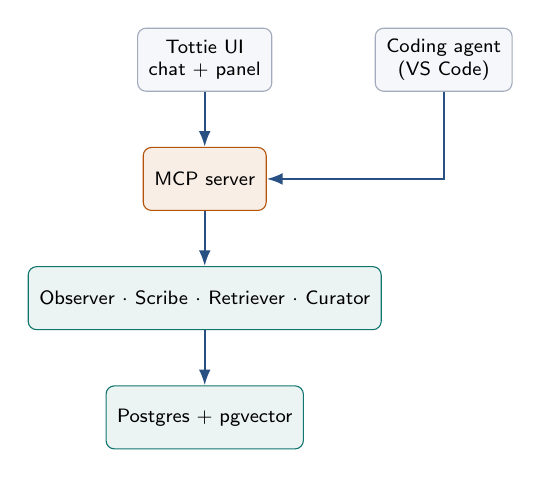
\begin{tikzpicture}[node distance=0.7cm]
      \node[bx] (ui) {Tottie UI\\chat + panel};
      \node[bx,right=1.3cm of ui] (ide) {Coding agent\\(VS Code)};
      \node[pbox,below=0.7cm of ui] (mcp) {MCP server};
      \node[abx,below=0.7cm of mcp] (core) {Observer $\cdot$ Scribe $\cdot$ Retriever $\cdot$ Curator};
      \node[abx,below=0.7cm of core] (db) {Postgres + pgvector};
      \draw[ar] (ui) -- (mcp);
      \draw[ar] (ide) |- (mcp);
      \draw[ar] (mcp) -- (core);
      \draw[ar] (core) -- (db);
    \end{tikzpicture}
  \end{figure}
  \begin{itemize}
    \item \textbf{Observer} --- is this worth remembering?
    \item \textbf{Scribe} --- structure, tag, embed, \textbf{reconcile}.
    \item \textbf{Retriever} --- runs every turn; find what is contextually relevant.
    \item \textbf{Curator} --- write the compact \textbf{Context Card} the agent receives.
  \end{itemize}
\end{frame}

% ---------- 6. Tiers ----------
\begin{frame}{The memory vault has tiers}
  \begin{tabularx}{\textwidth}{@{}l X@{}}
    \toprule
    \textbf{Tier} & \textbf{What it holds} \\
    \midrule
    Identity & Persona + permanent constraints. Pinned raw, zero search. \\
    Episodic & Chronological decisions, state changes, history. \\
    Knowledge & Ingested docs, files, references. \\
    Procedural (``Lessons'') & Mistake $\rightarrow$ solution pairs. Autosave. \\
    \bottomrule
  \end{tabularx}
  \vfill
  \begin{block}{Why tiers beat a flat vector store}
    Identity needs no search at all; episodic needs time; knowledge needs semantics; lessons need an
    error signature. One store, four retrieval policies.
  \end{block}
\end{frame}

% ---------- 7. The middle (card + probe) ----------
\begin{frame}{The part everyone leaves out: what reaches the model?}
  \textbf{Dual-path recall}: a card that is handed over automatically, plus a probe the agent can
  choose to run.
  \begin{block}{The Context Card (injected every turn)}
    \ttfamily\scriptsize
    [MEMORY CARD - 3 hits]\\[1mm]
    $\triangleright$ IDENTITY (pinned) user=Frans - girlfriend birthday = Nov 7\\
    $\triangleright$ EPISODIC 2026-10-29 decided: pgvector, not Qdrant \#tottie \#decision\\
    $\triangleright$ KNOWLEDGE (telecom-arch.pdf p.7) Server C behind A/B \#telecom \#infra\\
    $\rightarrow$ probe deeper: memory.probe("\#telecom")
  \end{block}
  \begin{itemize}
    \item \textbf{Ambient} --- the card is always there; the agent ``just knows.''
    \item \textbf{Deliberate} --- the card carries pointers; \texttt{memory.probe(tag)} opens the room.
  \end{itemize}
\end{frame}

% ---------- 8. Reconcile ----------
\begin{frame}{It changes its mind, correctly}
  \begin{block}{Contradiction at write time, not read time}
    ``I'm vegetarian now'' $\rightarrow$ the Scribe \textbf{supersedes} the old fact:
    old row $\texttt{valid\_to} = now$, new row $\texttt{valid\_from} = now$.
  \end{block}
  \begin{itemize}
    \item Retrieval filters \texttt{valid\_to IS NULL}, so a stale fact can never surface.
    \item Plain vector recall has \emph{no update semantics} --- both facts return and the model guesses.
    \item This is exactly LongMemEval's \emph{knowledge update} and MemoryAgentBench's \emph{conflict resolution}.
  \end{itemize}
\end{frame}

% ---------- 9. Three bodies ----------
\begin{frame}{One brain. Three bodies.}
  \begin{columns}
    \begin{column}{0.33\textwidth}
      \begin{block}{Tottie}
        Chat + reacting sprite. Remembers your \emph{life}.
      \end{block}
    \end{column}
    \begin{column}{0.33\textwidth}
      \begin{block}{Coding agent}
        Same MCP server in VS Code. Knows your \emph{stack}; autosaves fixes.
      \end{block}
    \end{column}
    \begin{column}{0.33\textwidth}
      \begin{block}{Memory Panel}
        The live X-ray. Watch it think.
      \end{block}
    \end{column}
  \end{columns}
  \vfill
  \centering
  \textbf{The money shot:} add a fact in the chat, then ask your coding agent --- it already knows.
\end{frame}

% ---------- 10. The panel ----------
\begin{frame}{The Memory Panel: the invisible, made visible}
  Real time, four blocks:
  \begin{enumerate}
    \item \textbf{Learning now} --- the turn + Observer verdict (KEEP/DISCARD, salience, reason).
    \item \textbf{Memories formed} --- \texttt{NEW} / \texttt{UPDATE} / \texttt{SUPERSEDE} / \texttt{SKIP}, with the text.
    \item \textbf{Inserted where} --- tier chip + tag/room chips + a growing room map.
    \item \textbf{Context injected} --- the exact card the model received this turn.
  \end{enumerate}
  \vfill
  \begin{block}{Why this is the hero}
    Judges should not have to take ``it remembers'' on faith. They watch the decision happen.
  \end{block}
\end{frame}

% ---------- 11. Proof ----------
\begin{frame}{We do not ask you to trust it. We measure it.}
  \begin{itemize}
    \item A \textbf{$\sim$40-item} suite across LongMemEval's categories (knowledge update, temporal,
    preference) plus contradiction resolution and abstention.
    \item Every item runs \textbf{memory ON vs OFF} --- the ablation that proves memory caused the answer.
    \item Metrics: answer accuracy, memory-hit@k, contradiction-correctness, tokens/query, p50/p95 latency.
  \end{itemize}
  \vfill
  \begin{alertblock}{The headline}
    \textbf{91\% lower p95 latency} and \textbf{90\% fewer tokens} than full-context, for a small
    accuracy trade --- the write-time curation argument, made falsifiable.
  \end{alertblock}
\end{frame}

% ---------- 12. What we built ----------
\begin{frame}{What was built during the Hackathon (Oct 27 -- Nov 4)}
  \begin{tabularx}{\textwidth}{@{}l X@{}}
    \toprule
    Component & \\
    \midrule
    \texttt{core/} & Memory engine: Observer, Scribe, Retriever, Curator; pgvector store; reconcile \\
    \texttt{mcp/} & MCP server: 6 tools, 2 resources, the context-card prompt \\
    \texttt{ui/} & Tottie chat, sprite state machine, live Memory Panel, ablation toggle \\
    \texttt{eval/} & ON/OFF ablation harness \\
    \texttt{docs/} & Full architecture + flows + this deck (LaTeX $\rightarrow$ PDF) \\
    \bottomrule
  \end{tabularx}
  \vfill
  \centering\small Every component is committed on a dated branch; the ledger is in
  \texttt{docs/business/hackathon\_compliance}.
\end{frame}

% ---------- 13. The joke + pitch ----------
\begin{frame}{So what did I actually build it for?}
  \begin{center}
    \Large ``Everything I was mad at my girlfriend for ---\\ and the one thing that matters: her birthday.''
  \end{center}
  \vfill
  \begin{itemize}
    \item \textbf{Autosave} --- an agent makes a mistake once, and never again.
    \item \textbf{A personal AI} that actually knows you, not just your last 20 messages.
    \item \textbf{The company brain} --- remember that Server C sits behind A and B before designing it.
  \end{itemize}
\end{frame}

% ---------- 14. Close ----------
\begin{frame}[plain]
  \begin{center}
    \Huge Tottie\\[3mm]
    \large It just remembers.\\[6mm]
    \normalsize github.com/frans-nekongo/Tottie
  \end{center}
\end{frame}

\end{document}
